\section{Теоретическая часть}

В сравнение будут участвовать два распространённых сканера уязвимостей - XSpider от компании Positive Technologies и Nessus от Tenable.

Сравнивать возможности сканеров будем в виртуальной сети, выделив одну машину для жертвы и одну для сканера. В качестве жертвы будем использовать известный образ Metasploitable 2 от Rapid7.

\subsection{XSpider}

Из открытых источников получилось найти только документ, названный "Краткое описание продукта". Если убрать из него всю маркетинговую составляющую, то заявленные функции выглядят так:

\begin{itemize}
\item Контроль изменений на сканируемых узлах, дающий полную картину защищенности в динамике.
­\item Инвентаризация всех сетевых устройств в организации.
­\item Эвристический метод определения типов и имен сервисов (HTTP, FTP, SMTP, POP3, DNS, SSH и др.) даже на нестандартных портах.
­\item Обработка RPC-сервисов (Windows и *nix) с полной идентификацией, включая точное определение конфигурации компьютера.
­\item Проверка слабости парольной защиты: оптимизированный подбор паролей практически во всех сервисах, требующих аутентификации.
­\item Глубокий анализ веб-сайтов, включая выявление уязвимостей: SQLi, XSS, запуск произвольных программ и др.
­\item Анализ структуры HTTP-серверов для поиска слабых мест в конфигурации.
­\item Расширенная проверка узлов под управлением Windows.
­\item Проведение проверок на нестандартные DoS-атаки.	
\end{itemize}

\begin{figure}[H]
	\centering
	\caption{Логика использования ПО XSpider}
	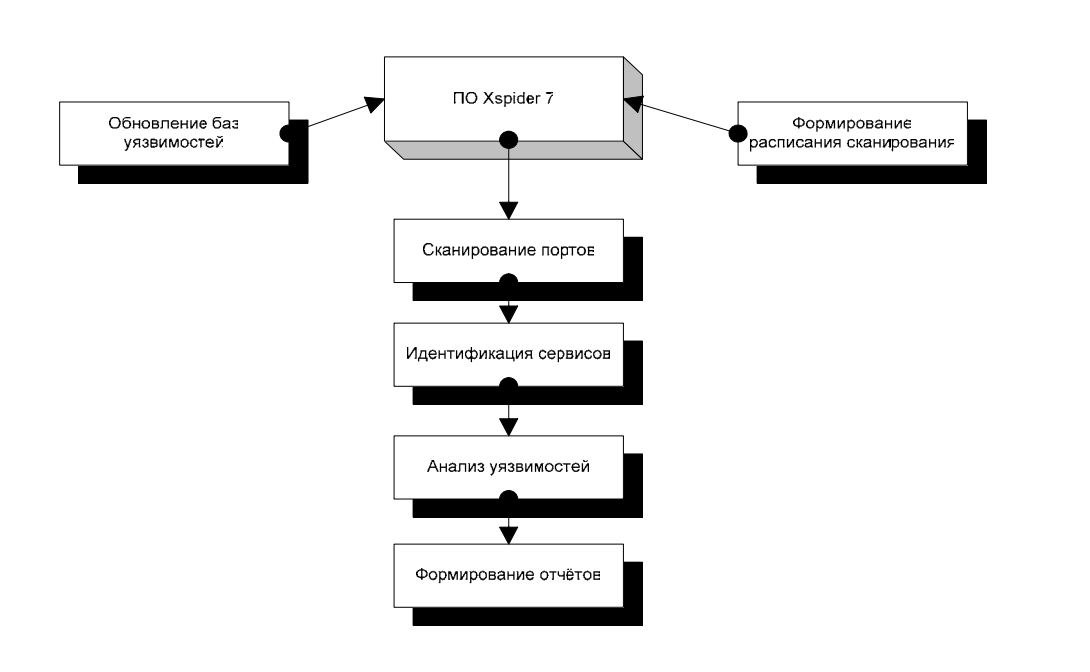
\includegraphics[width=.9\textwidth]{img/spider.png}
\end{figure}


\subsection{Nessus}

 Про Nessus последней версии вообще нет документации на русском языке. Функциональность расширяется за счёт плагинов, но в тестируемой версии (Home Edition) были заявлены все те же возможности, что и у XSpider.
 
 
 \subsection{Методика и критерии выставления оценок}
 
 Образ Metasploitable 2 достаточно старый, поэтому странно, если какие-то уязвимости не будут найдены.
 
 За каждый сервис будем давать 3 очка, если найдена высокая уязвимость, 2, если средняя и 1 если минорная. Надо бы ставить -5 баллов за каждый нераспознанный сервис, но тогда вообще в минус уйдём.
